\subsubsection{feature::input\_item\_info::InputItemInfoView}

\label{feature::input_item_info::InputItemInfoView}
\begin{figure}[ht]
	\centering
	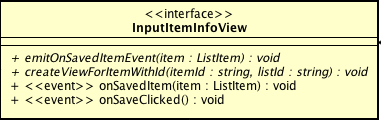
\includegraphics[scale=0.5]{Sezioni/SottosezioniST/img/app/InputItemInfoView.png}
	\caption{feature::input\_item\_info::InputItemInfoView}
\end{figure}

\begin{itemize}
\item \textbf{Descrizione}: Questa interfaccia rappresenta la view relativa all'input delle informazioni di un oggetto della lista-spesa.
\item \textbf{Utilizzo}: L'interfaccia viene utilizzata per disaccoppiare presenter e implementazione dell'aggiunta, visualizza i dati che gli vengono passati dal presenter.
\item \textbf{Attributi}:
\item \textbf{Metodi}:
	\begin{itemize}
	\item \textit{public emitOnSavedItemEvent(item:ListItem):void}\\
	Metodo che permette l'emissione dell'evento \texttt{OnSavedItemEvent}.
			\\ \textbf{Parametri}: \begin{itemize}
			\item \textit{item:ListItem}\\
			Oggetto rappresentante tutte le informazioni inserite dall'utente.
			\end{itemize} 
	\item \textit{public createViewForItemWithId(itemId:string,listId:string):void}\\
	Il metodo crea una view per l'inserimento delle informazioni di un oggetto precompilando i campi già inseriti con le informazioni ottenute a partire dal suo id.
			\\ \textbf{Parametri}: \begin{itemize}
			\item \textit{itemId:string}\\
			L'id dell'oggetto del quale si vogliono utilizzare le informazioni.
			\item \textit{listId:string}\\
			L'id della lista a cui appartiene l'oggetto da modificare.
			\end{itemize} 
	\end{itemize}
\item \textbf{Eventi}:
\begin{itemize}
\item \textit{public onSavedItem(item:ListItem):void}\\
Evento che rappresenta il salvataggio dei dati di un particolare oggetto della lista-spesa.
			\\ \textbf{Parametri}: \begin{itemize}
			\item \textit{item:ListItem}\\
			L'oggetto della lista che è stato salvato.
			\end{itemize} 
\item \textit{public onSaveClicked():void}\\
Evento che rappresenta il click dell'utente sulla componente grafica necessaria al salvataggio dei dati immessi.
\end{itemize}
\end{itemize}

\subsubsection{feature::input\_item\_info::view::InputItemInfoViewImpl}

\label{feature::input_item_info::view::InputItemInfoViewImpl}
\begin{figure}[ht]
	\centering
	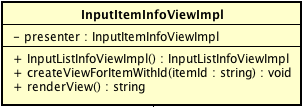
\includegraphics[scale=0.5]{Sezioni/SottosezioniST/img/app/InputItemInfoViewImpl.png}
	\caption{feature::input\_item\_info::view::InputItemInfoViewImpl}
\end{figure}

\begin{itemize}
\item \textbf{Descrizione}: Questa classe rappresenta la componente grafica necessaria all'inserimento delle informazioni di un oggetto di una lista-spesa, implementando l'interfaccia InputItemInfoView.
\item \textbf{Utilizzo}: Questa classe viene utilizzata dall'utente ogniqualvolta aggiunge o modifica i dati di un oggetto all'interno di una lista-spesa.
\item \textbf{Attributi}:
	\begin{itemize}
	\item \textit{private presenter:InputItemViewPresenter}\\
	Il presenter associato all'aggiunta o alla modifica dei dati di un oggetto alla lista, al quale questa classe delega la gestione del comportamento dell'elemento di inserimento.
	\end{itemize}
\item \textbf{Metodi}:
	\begin{itemize}
	\item \textit{InputItemInfoViewImpl():InputItemInfoViewImpl}\\
	Il costruttore della classe InputItemInfoViewImpl.
	\item \textit{public createViewForItemWithId(itemId:string,listId:string):void}\\
	Il metodo crea una view per l'inserimento delle informazioni di un oggetto precompilando i campi già inseriti con le informazioni ottenute a partire dal suo id.
			\\ \textbf{Parametri}: \begin{itemize}
			\item \textit{itemId:string}\\
			L'id dell'oggetto del quale si vogliono utilizzare le informazioni.
			\item \textit{listId:string}\\
			L'id della lista a cui appartiene l'oggetto da modificare.
			\end{itemize} 
	\item \textit{public renderView():string}\\
	Genera il codice HTML CSS JS necessario per visualizzare la componente grafica della lista-spesa necessaria all'inserimento delle informazioni di un oggetto nella lista.
	\end{itemize}
\item \textbf{Eventi}:
\end{itemize}

\subsubsection{feature::input\_item\_info::presenter::InputItemInfoViewPresenter}

\label{feature::input_item_info::presenter::InputItemInfoViewPresenter}
\begin{figure}[ht]
	\centering
	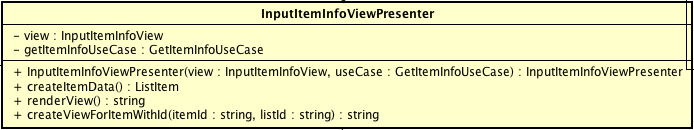
\includegraphics[scale=0.5]{Sezioni/SottosezioniST/img/app/InputInfoViewPresenter.png}
	\caption{feature::input\_item\_info::presenter::InputItemInfoViewPresenter}
\end{figure}

\begin{itemize}
\item \textbf{Descrizione}: Questa classe rappresenta il presenter per gli elementi di aggiunta dei dati degli oggetti di una lista-spesa.
\item \textbf{Utilizzo}: Il presenter fa da tramite tra l'implementazione dell'elemento di aggiunta dei dati e la view, formattando i dati che verranno visualizzati nella view e manipolando gli input dell'utente per eseguire le operazioni predisposte.
\item \textbf{Attributi}: 
	\begin{itemize}
	\item \textit{private view:InputItemInfoView}\\
	La view associata al presenter.
	\item \textit{private getItemInfoUseCase:GetItemInfoUseCase}\\
	Elemento di contatto con il database attraverso il quale si possono ottenere da quest'ultimo i dati relativi a un particolare oggetto.
	\end{itemize}
\item \textbf{Metodi}:
	\begin{itemize}
	\item \textit{public createItemData():ListItem}\\
	Crea l'oggetto che contiene i dati di un singolo oggetto della lista, prendendo i dati da ciò che l'utente ha inserito nella vista
	\item \textit{public renderView():string}\\
	Genera il codice HTML CSS JS necessario per visualizzare la componente grafica della lista-spesa necessaria all'inserimento delle informazioni di un oggetto nella lista.
	\item \textit{public createViewForItemWithId(itemId:string):void}\\
	Il metodo crea una view per l'inserimento delle informazioni di un oggetto precompilando i campi già inseriti con le informazioni ottenute a partire dal suo id.
			\\ \textbf{Parametri}: \begin{itemize}
			\item \textit{itemId:string}\\
			L'id dell'oggetto del quale si vogliono utilizzare le informazioni.
			\item \textit{listId:string}\\
			L'id della lista a cui appartiene l'oggetto da modificare.
			\end{itemize} 
	\item \textit{public InputInfoViewPresenter(view:InputItemInfoView, useCase:GetItemInfoUseCase):InputInfoViewPresenter}\\
	Il costruttore della classe InputInfoViewPresenter.
				\\ \textbf{Parametri}: \begin{itemize}
				\item \textit{view:InputItemInfoView}\\
				La view necessaria alla costruzione del presenter.
				\item \textit{useCase:GetItemInfoUseCase}\\
				L'elemento di interfaccia con il database.
			\end{itemize} 
	\end{itemize}
\item \textbf{Eventi}:
\end{itemize}

\subsubsection{usecase::GetItemInfoUseCase}

\label{usecase::GetItemInfoUseCase}
\begin{figure}[ht]
	\centering
	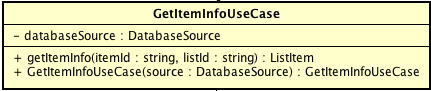
\includegraphics[scale=0.5]{Sezioni/SottosezioniST/img/app/GetItemInfoUseCase.png}
	\caption{usecase::GetItemInfoUseCase}
\end{figure}

\begin{itemize}
\item \textbf{Descrizione}: Classe che permette di ottenere i dati relativi ad un oggetto all'interno della lista salvato nel database.
\item \textbf{Utilizzo}: Se le classi necessitano di comunicare con il database e ricevere informazioni su un particolare oggetto, dovranno passare attraverso questa classe.
\item \textbf{Attributi}: 
	\begin{itemize}
	\item \textit{private databaseSource:DatabaseSource}\\
	Database con il quale questa classe dialoga.
	\end{itemize}
\item \textbf{Metodi}:
	\begin{itemize}
	\item \textit{public getItemInfo(itemId:string,listId):ListItem}\\
	Ritorna l'oggetto della lista spesa richiesto.
			\\ \textbf{Parametri}: \begin{itemize}
			\item \textit{itemId:string}\\
			L'id dell'oggetto del quale si vogliono ottenere le informazioni.
			\item \textit{listId:string}\\
			L'id della lista-spesa nella quale si trova l'oggetto in questione.
			\end{itemize} 
			\item \textit{public GetItemInfoUseCase(source:DatabaseSource):GetItemInfoUseCase}\\
			Il costruttore della classe GetItemInfoUseCase.
				\\ \textbf{Parametri}: \begin{itemize}
				\item \textit{source:DatabaseSource}\\
				Il database necessario alla costruzione dell'oggetto.
			\end{itemize} 
	\end{itemize}
\item{Eventi}:
\end{itemize}

\subsubsection{feature::modify\_item::ModifyItemView}

\label{feature::modify_item::ModifyItemView}
\begin{figure}[ht]
	\centering
	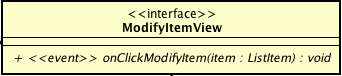
\includegraphics[scale=0.5]{Sezioni/SottosezioniST/img/app/ModifyItemView.png}
	\caption{feature::modify\_item::ModifyItemView}
\end{figure}

\begin{itemize}
\item \textbf{Descrizione}: Questa interfaccia rappresenta la view relativa alla modifica delle informazioni di un oggetto alla lista-spesa.
\item \textbf{Utilizzo}: L'interfaccia viene utilizzata per disaccoppiare presenter e implementazione della modifica, visualizza i dati che gli vengono passati dal presenter.
\item \textbf{Attributi}: 
\item \textbf{Metodi}:
\item \textbf{Eventi}:
	\begin{itemize}
	\item \textit{public onClickModifyItem(item:ListItem):void}\\
	Evento che rappresenta il salvataggio dei dati immessi.
			\\ \textbf{Parametri}: \begin{itemize}
			\item \textit{item:ListItem}\\
			Oggetto contenente tutti i dati immessi e salvati da parte dell'utente.
			\end{itemize} 
	\end{itemize}
\end{itemize}

\subsubsection{feature::modify\_item::view::ModifyItemViewImpl}

\label{feature::modify_item::view::ModifyItemViewImpl}
\begin{figure}[ht]
	\centering
	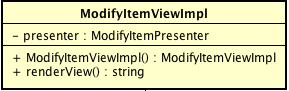
\includegraphics[scale=0.5]{Sezioni/SottosezioniST/img/app/ModifyItemViewImpl.png}
	\caption{feature::modify\_item::view::ModifyItemViewImpl}
\end{figure}

\begin{itemize}
\item \textbf{Descrizione}: Questa classe rappresenta la componente grafica necessaria alla modifica delle informazioni di un oggetto di una lista-spesa, implementando l'interfaccia ModifyItemInfoView.
\item \textbf{Utilizzo}: Questa classe viene utilizzata dall'utente ogniqualvolta modifica i dati di un oggetto all'interno di una lista-spesa.
\item \textbf{Attributi}: 
	\begin{itemize}
	\item \textit{private presenter:ModifyItemPresenter}\\
	Il presenter associato all'aggiunta dei dati di un oggetto alla lista, al quale questa classe delega la gestione del comportamento dell'elemento di inserimento.
	\end{itemize}
\item \textbf{Metodi}:
	\begin{itemize}
	\item \textit{public ModifyItemViewImpl():ModifyItemViewImpl}\\
	Il costruttore della classe ModifyItemViewImpl.
	\item \textit{public renderView():string}\\
	Genera il codice HTML CSS JS necessario per visualizzare la componente grafica della lista-spesa necessaria alla modifica delle informazioni di un oggetto nella lista.
	\end{itemize}
\item \textbf{Eventi}:
\end{itemize}

\subsubsection{feature::modify\_item::presenter::ModifyItemViewPresenter}

\label{feature::modify_item::presenter::ModifyItemViewPresenter}
\begin{figure}[ht]
	\centering
	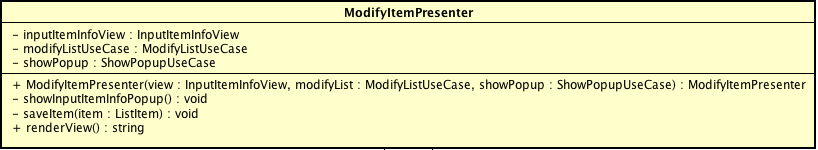
\includegraphics[scale=0.5]{Sezioni/SottosezioniST/img/app/ModifyItemPresenter.png}
	\caption{feature::modify\_item::presenter::ModifyItemViewPresenter}
\end{figure}

\begin{itemize}
\item \textbf{Descrizione}: Questa classe rappresenta il presenter per la vista dedicata alla modifica dei dati di un oggetto presente all'interno di una lista.
\item \textbf{Utilizzo}: Il presenter fa da tramite tra l'implementazione dell'elemento di aggiunta dei dati e la view, formattando i dati che verranno visualizzati nella view e manipolando gli input dell'utente per eseguire le operazioni predisposte.
\item \textbf{Attributi}: 
	\begin{itemize}
	\item \textit{private inputItemInfoView:InputItemInfoView}\\
	La view associata al presenter.
	\item \textit{private modifyListUseCase:ModifyListUseCase}\\
	Elemento dedito alla modifica dei dati di un oggetto all'interno del database.
	\item \textit{private showPopup:ShowPopupUseCase}\\
	Componente necessaria alla visualizzazione di modali.
	\end{itemize}
\item \textbf{Metodi}:
	\begin{itemize}
	\item \textit{public ModifyItemPresenter(view:InputItemInfoView, modifyList:ModifyListUseCase, \\ showPopup:ShowPopupUseCase):ModifyItemPresenter}\\
	Il costruttore della classe ModifyItemViewPresenter
		\\ \textbf{Parametri}: \begin{itemize}
		\item \textit{view:InputItemInfoView}\\
		La view associata al presenter.
		\item \textit{modifyList:ModifyListUseCase}\\
		L'elemento di contatto con il database.
		\item \textit{showPopup:ShowPopupUseCase}\\
		Componente necessaria alla visualizzazione di modali.
		\end{itemize} 
	\item \textit{private showInputItemInfoPopup():void}\\
	Il metodo mostra un modale per l'inserimento delle informazioni relative ad un oggetto della lista-spesa.
	\item \textit{private saveItem(item:ListItem):string}\\
	Metodo usato per salvare i dati di un oggetto dopo la modifica.
			\\ \textbf{Parametri}: \begin{itemize}
			\item \textit{item:ListItem}\\
			L'oggetto del quale si vogliono salvare le modifiche.
			\end{itemize} 
	\item \textit{public renderView():string}\\
		Genera il codice HTML CSS JS necessario per visualizzare la componente grafica della lista-spesa necessaria alla modifica delle informazioni di un oggetto nella lista.
	\end{itemize}
\item \textbf{Eventi}:
\end{itemize}